\section{Nearest Counterfactual Explanations}\label{sec:generation}
In this section, two main approaches of the nearest CF are introduced. One of them is the gradient-based algorithm, which has become the majority since \citeauthor{watcher2017} \cite{watcher2017} have purposed their first loss function \cite{CFReview}. However, gradient-based methods can only handle differentiable models. For supplements, the genetic method is also introduced.
%统一字母代号:
% K是特征,feature channel
% N是样本 instances
% D是什么?
% i 分类类别

\subsection{Gradient-based Method}\label{sec:lossFunc}
CF explanation focuses on which kind of minimal perturbation in the data subject will leads to a different classification. Therefore, the search of a an appropriate CF example is boiled down to an optimizing problem with at least two requirements: (1.) classified as the counter class, and (2.) still similar to the original data with only necessary modifications. \citeauthor{watcher2017} \cite{watcher2017} has proposed the following formula, which becomes the basis of the following research:
\begin{equation}\label{eq:watcher}
  \textbf{c}=\arg\min_{\textbf{c}}target\_loss(f(\textbf{c}),y)+d(\textbf{x,c})
\end{equation}
where \textbf{x} is the original data, y is the target data class, \textbf{c} is the generated counterfactual data, and f is the model so that f(\textbf{c}) is the new prediction of the model, i.e. the new class. The first part of the formula encourages a different class, while the second part penalizes large distances away from the original data. According to \citeauthor{watcher2017}'s notation, the first part is called ``validity'' and the second part is ``proximity'', both have significant impacts on final results \cite{watcher2017}.

\subsubsection{Proximity Term} Proximity measures how close is the CF with its original subject. Another main contribution of \cite{watcher2017} is to define distance as \emph{$L_1$} norm divided by MAD (median absolute deviation):
\begin{equation}\label{eq:distMAD}
  dist = \sum_{k=1}^{K}\frac{|\textbf{x-c}|}{MAD_k}
\end{equation}
where MAD is defined for every feature k over the whole points set P:
\begin{equation}\label{eq:MAD}
  MAD_k=median_{i\in P}(|{X_{i,k}}-median_{j\in P}(X_{j,k})|)
\end{equation}
The \emph{$L_1$} norm in \autoref{eq:distMAD} prones to generate zero entries, which ensures a sparse optimizing result. Normalising the norm is important as well, otherwise big range data would have heavy weights. Here MAD turns out to outperform standard deviation, because it cooperates with \emph{$L_1$} norm better, and generates even more sparse result.

Sometimes data may contain categorical features (e.g. occupation, gender\dots), it is counter-intuitive to define ``distance'' for these features. A simple matching distance is able to cope with the issue, where distance 1 is assigned to value changes and 0 if the value remains unchanged \cite{DiCE}.
\begin{equation}\label{eq:distCate}
  dist\_cat(\textbf{c,x})=\sum_{k=1}^{K_{cat}}\mathbb{I}(c^k\neq x^k)
\end{equation}
Combining equation \ref{eq:distMAD} and \ref{eq:distCate} weighted by the number of continuous and categorical features, the most common used distance metric is shown as following:
\begin{equation}\label{eq:distCombined}
  d(\textbf{x,c})=\frac{1}{K_{con}}\sum_{k=1}^{K_{con}}\frac{|\textbf{x-c}|}{MAD_k}
  +\frac{1}{K_{cat}}\sum_{k=1}^{K_{cat}}\mathbb{I}(\textbf c^k
  \neq \textbf x^k)
\end{equation}

\subsubsection{Validity Term} Validity measures the ratio of the CFs that successfully obtained the desired class label \cite{CFReview}. For simplicity, the following context assumes the original class label to be 0, and the desired label to be 1 for binary classification. The prediction of the model f(\textbf{c}) is a continuous value between 0 and 1. One of the choices of the target loss term is the \emph{$L_2$} norm $(f(\textbf{c})-y)^2$ \cite{watcher2017}. \citeauthor{DiCE} \cite{DiCE} argue that a valid counterfactual suffices if it bypasses the classification threshold of the model (typically 0.5), but the \emph{$L_2$} norm always prefer the extreme value 1. The underlying issue is that counterfactuals, unless predicted exactly as 1, still receives penalty even if it is classified correctly. A better choice is the hinge-loss, which does not penalize as long as the prediction exceeds a certain threshold, see \autoref{fig:hingeloss}.
\begin{equation}\label{eq:hingeloss}
  hinge\_trgtloss=\max(0,1-logit(f(\textbf{c})))
\end{equation}
where \emph{logit(f(\textbf{c}))} is the final activation before entering a sigmoid/softmax output layer. This loss function, however, requires internal logits of the model, therefore is not available under a ``black-box'' situation.
\begin{figure}
  \centering
  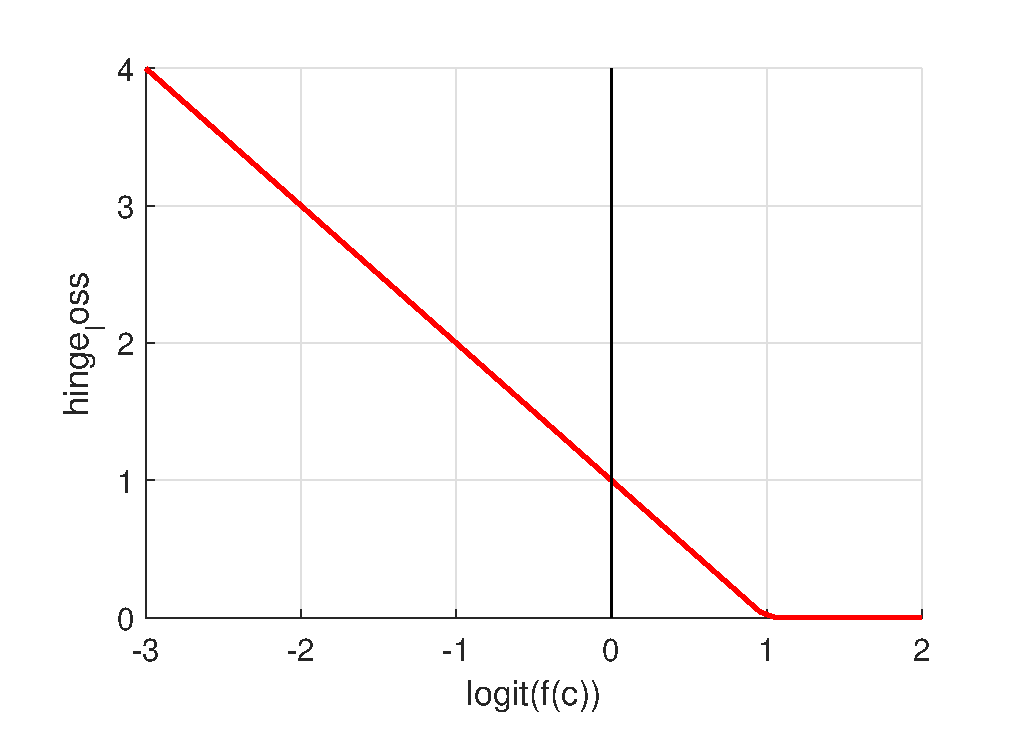
\includegraphics[width=0.5\textwidth]{hingeloss.eps}
  \caption{the hinge loss penalize wrong classification heavily, correct one near the boundary slightly and has no effect above a certain threshold}\label{fig:hingeloss}
\end{figure}

So far the equations are derived for a binary classification problem, where a ``why A not $\neg${A}'' or ``why A not B'' question is raised. For n-ary classification, where the prediction output is a n-length vector, \citeauthor{prototype} \cite{prototype} mentioned the following formula:
\begin{equation}\label{eq:lossPred}
  predloss=\max([f(\textbf{c})]_{i=i_0}-\max_{i\neq i_0}[f(\textbf{c})]_i),-\kappa)
\end{equation}
where $i_0=\arg\max f(\textbf{x})$ is the original data label, and $[f(\textbf{c})]_i$ is the i-th class prediction probability. This loss function gives a negative value if the predicted class is different than the original class, and $-\kappa < 0$ caps the negative value.

Now, \autoref{eq:watcher} is already able to generate counterfactuals. However, it turns out that sometimes the given CF is hard to interpret and not actionable. Details of the issue are kept for \autoref{sec:adversarial}. To deal with the issue, some additional terms could be appended to the above equation to improve performance.
